
%----------------------------------------------------------------------------------------
%	Lecture 7
%----------------------------------------------------------------------------------------

\chapter{First-order Linear with Constant Coefficients: Behavior of Solutions, Use of Complex Methods} 

\bigbreak

\section{First Order Linear Equations with Constant Coefficients}

Earlier, we saw how to solve a First Order Linear Differential Equation. 
And we got a general solution for it as :

$$ y = e^{-\int p(t)dt } \int q(t) e^{\int p(t) dt} dt + ce^{- \int p(t) dt} $$

Now if we take $p(t) = k$ to be constant then our solution becomes,

$$ y = e^{-kt} \int q(t) e^{kt} dt + ce^{-kt} $$

If $k > 0$ then the second term goes to zero as $t \to \infty$, and the second term is a function and is called the Steady State Solution.

As $t \to \infty$, all other solution approach the steady state solution.

\begin{figure}[ht!]
    \centering
    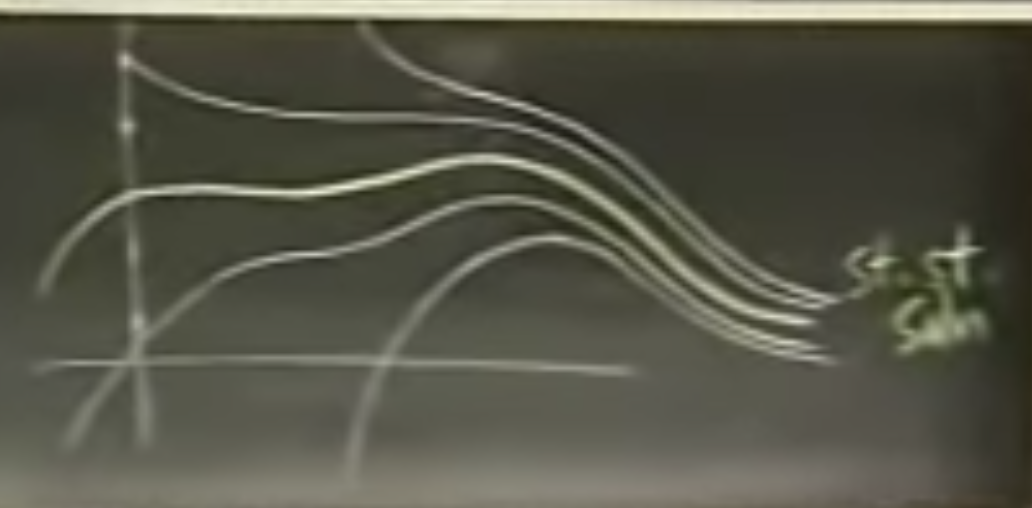
\includegraphics[scale=0.5]{./images/lecture_7_figure_1.png}
    \caption{Steady State Solution}
\end{figure}

All curves have the same property that they are trying to get closer to the other curves.
Thus, there is nothing special about the steady state solution.

Here, we see $y(t)$ as the response of the system with the input $q(t)$ as that is the only independent term in our solution.
Our steady state solution is the solution where the transient term is zero.

\subsection{Superposistion Principle}

For any two steady state solutions, the following holds.

If $q_1(t)$ produces a response of $y_1(t)$ 
and $q_2(t)$ produces a response of $y_2(t)$ 
then $q_1(t) + q_2(t)$ produces a response of $y_1(t) + y_2(t)$.

This can be proved by just adding the equation of $y_1(t)$ and $y_2(t)$.

Also, if $q(t)$ produces a response of $y(t)$ 
then $cq(t)$ produces a response $cy(t)$.


\subsection{Trigonometric Inputs}

If $q(t) = \cos \omega t$ then our equation is $y' + ky = k \cos \omega t$.
Here, $\omega$ is called the angular frequency.
It is the number of complete oscillations in the distance $2 \pi$.

We're going to solve it using complex numbers since it is easier to integrate exponentials.
Our equation becomes $\tilde{y}' + k\tilde{y} = k e^{i \omega t}$
where $\tilde{y}$ is the complex solution to this equation and $y(t)$ is the real part of this solution.

Here, our integraing factor is $e^{kt}$.
Mutliplying both sides, we get, 

\begin{align*}
    \tilde{y}' e^{kt} + k e^{kt} y & = k e^{i \omega t + kt} \\
    (\tilde{y} e^{kt})' & = k e^{(i \omega + k) t} \\
    \tilde{y} e^{kt} & =\frac{k}{i \omega + k} e^{(i \omega + k) t} \\
    \tilde{y} & = \frac{1}{1 + i \frac{w}{k}} e^{iwt}
\end{align*}

Converting the above to polar form, we get, 

$$ 1 + i \frac{\omega}{k} = \left( \sqrt{ 1 + \left( \frac{\omega}{k} \right)^2 } \right) e^{i \phi} $$

where $\tan \phi = \frac{\omega}{k}$. Thus, 

$$ \tilde{y} = \frac{1}{\sqrt{ 1 + \left( \frac{\omega}{k} \right)^2 }} e^{i \omega t - i \phi} $$

Taking the real part of it we'll get, 

$$ y(t) = \frac{1}{\sqrt{ 1 + \left( \frac{\omega}{k} \right)^2 }} \cos(\omega t - \phi) $$

Here, $\phi = \arctan \left( \frac{\omega}{k} \right)$ and it is called the phase lag of the function.

If $k$ is increasing then then $\frac{\omega}{k}$ is going down.
Thus, the amplitude is increasing and the phase lag is decreasing.

